\begin{frame}[fragile]{Tutorial: One-site operators}

\begin{columns}

\begin{column}{4.5cm}

\begin{onlyenv}<1->
\begin{lstlisting}[language=JuliaLocal, style=julia, basicstyle=\small]
XZp = X * Zp

inner(Zm, XZp)

inner(Zm', XZp)
inner(Zp', XZp)
\end{lstlisting}
\end{onlyenv}

\begin{onlyenv}<3->
\begin{lstlisting}[language=JuliaLocal, style=julia, basicstyle=\small]
(dag(Zm)' * X * Zp)[]
inner(Zm', X, Zp)

XZp = apply(X, Zp)
inner(Zm, XZp)
\end{lstlisting}
\end{onlyenv}

\end{column}

\begin{column}{4.5cm}

\begin{onlyenv}<1-1>
X|Z+$\rangle$ = |Z-$\rangle$ \\
~\\
error: not a scalar value \\
~\\
$\approx$ 1 \\
$\approx$ 0
\end{onlyenv}

\begin{onlyenv}<2->
\vspace*{0.0cm}
\begin{center}

\includegraphics[width=1.0\textwidth]{
  slides/assets/XZp.png
} \\

\includegraphics[width=1.0\textwidth]{
  slides/assets/outer_XZp_Zm.png
} \\
=

\includegraphics[width=1.0\textwidth]{
  slides/assets/outer_Zm_Zm.png
} \\

\includegraphics[width=1.0\textwidth]{
  slides/assets/ZmXZp.png
} \\
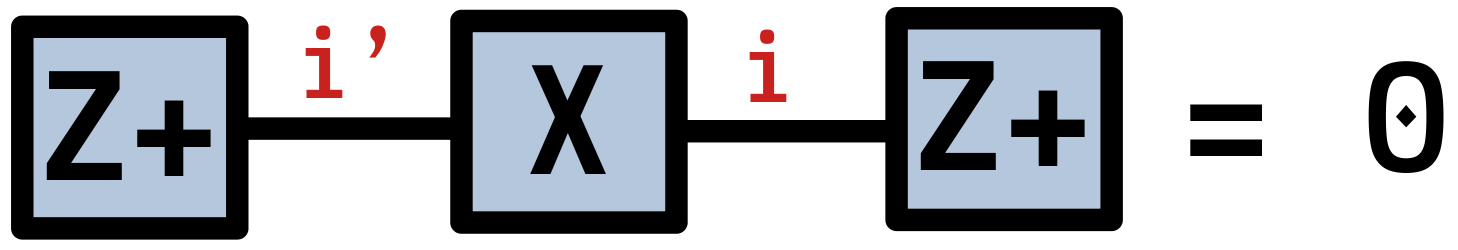
\includegraphics[width=1.0\textwidth]{
  slides/assets/ZpXZp.png
}
\end{center}
\vspace*{0.0cm}
\end{onlyenv}

\begin{onlyenv}<3-3>
$\approx$ 1 \\
$\approx$ 1 \\
~\\
= noprime(X * Zp) \\
$\approx$ 1 \\
\end{onlyenv}

\begin{onlyenv}<4->
\vspace*{0.0cm}
\begin{center}
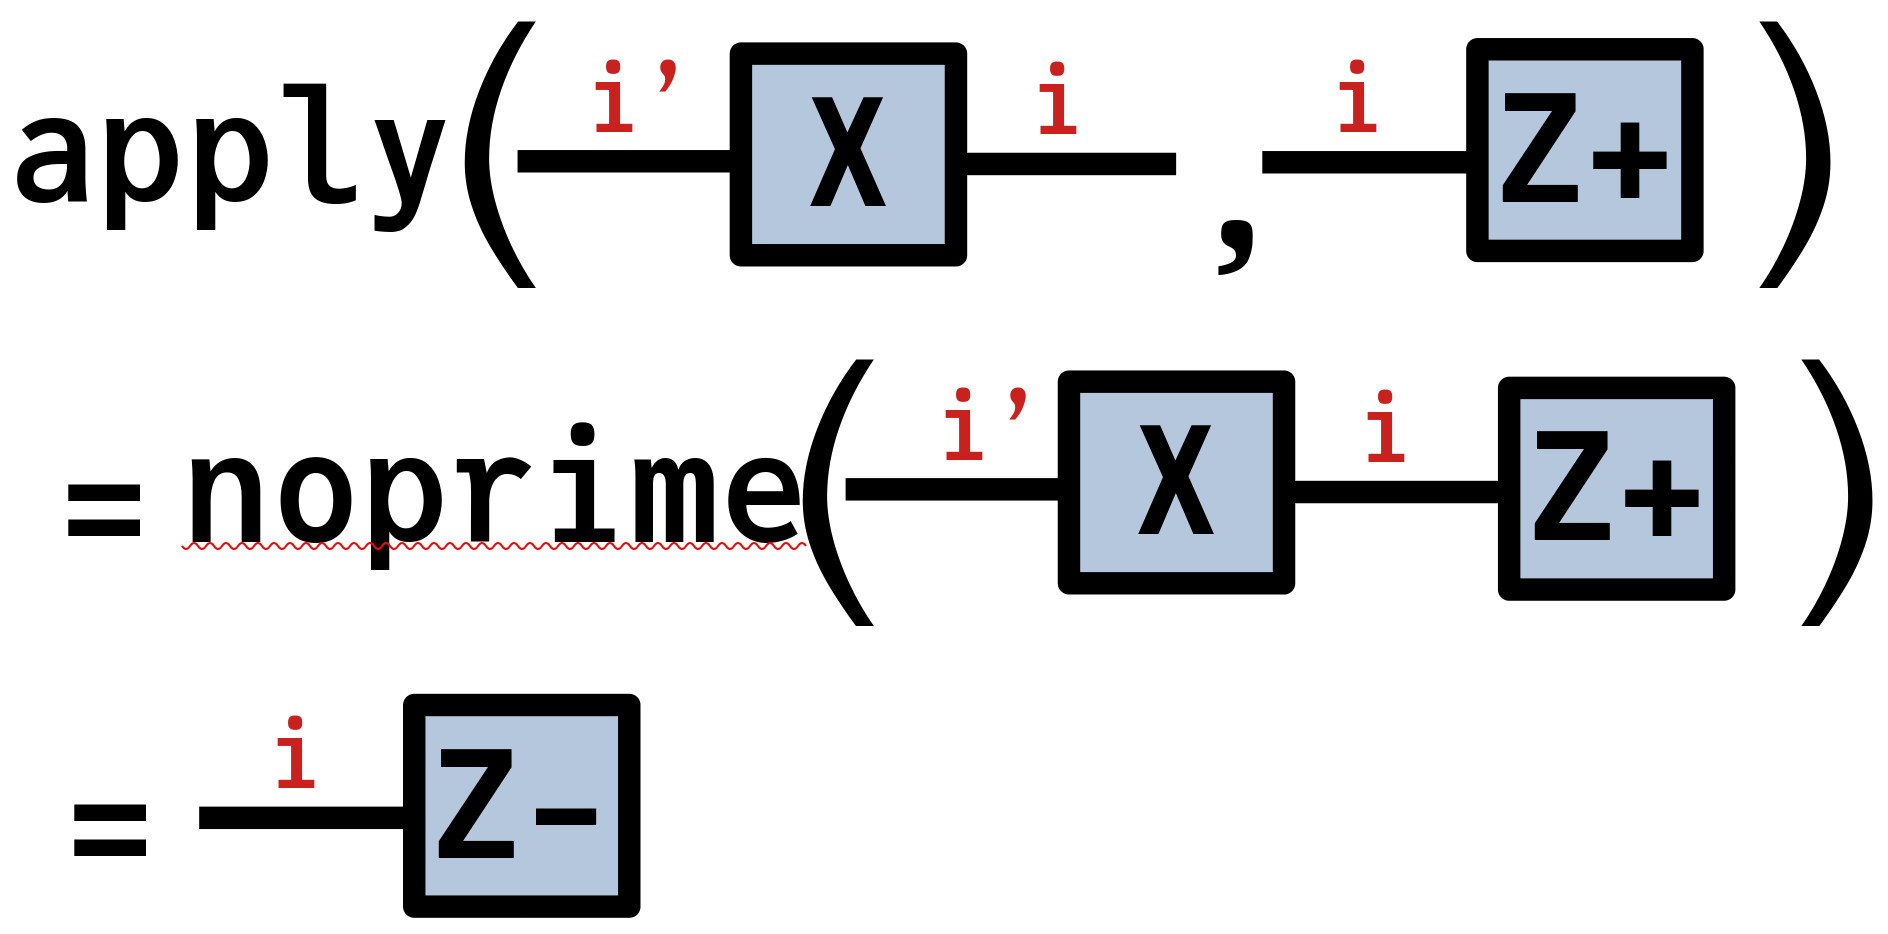
\includegraphics[width=1.0\textwidth]{
  slides/assets/apply_XZp.png
}
\end{center}
\vspace*{0.0cm}
\end{onlyenv}

\end{column}

\end{columns}

\end{frame}
